% Figure S1. Cartoon representation of tb1 locus
%-------------------------------------------------------------------
\begin{figure*}[!t]
  \begin{center}
   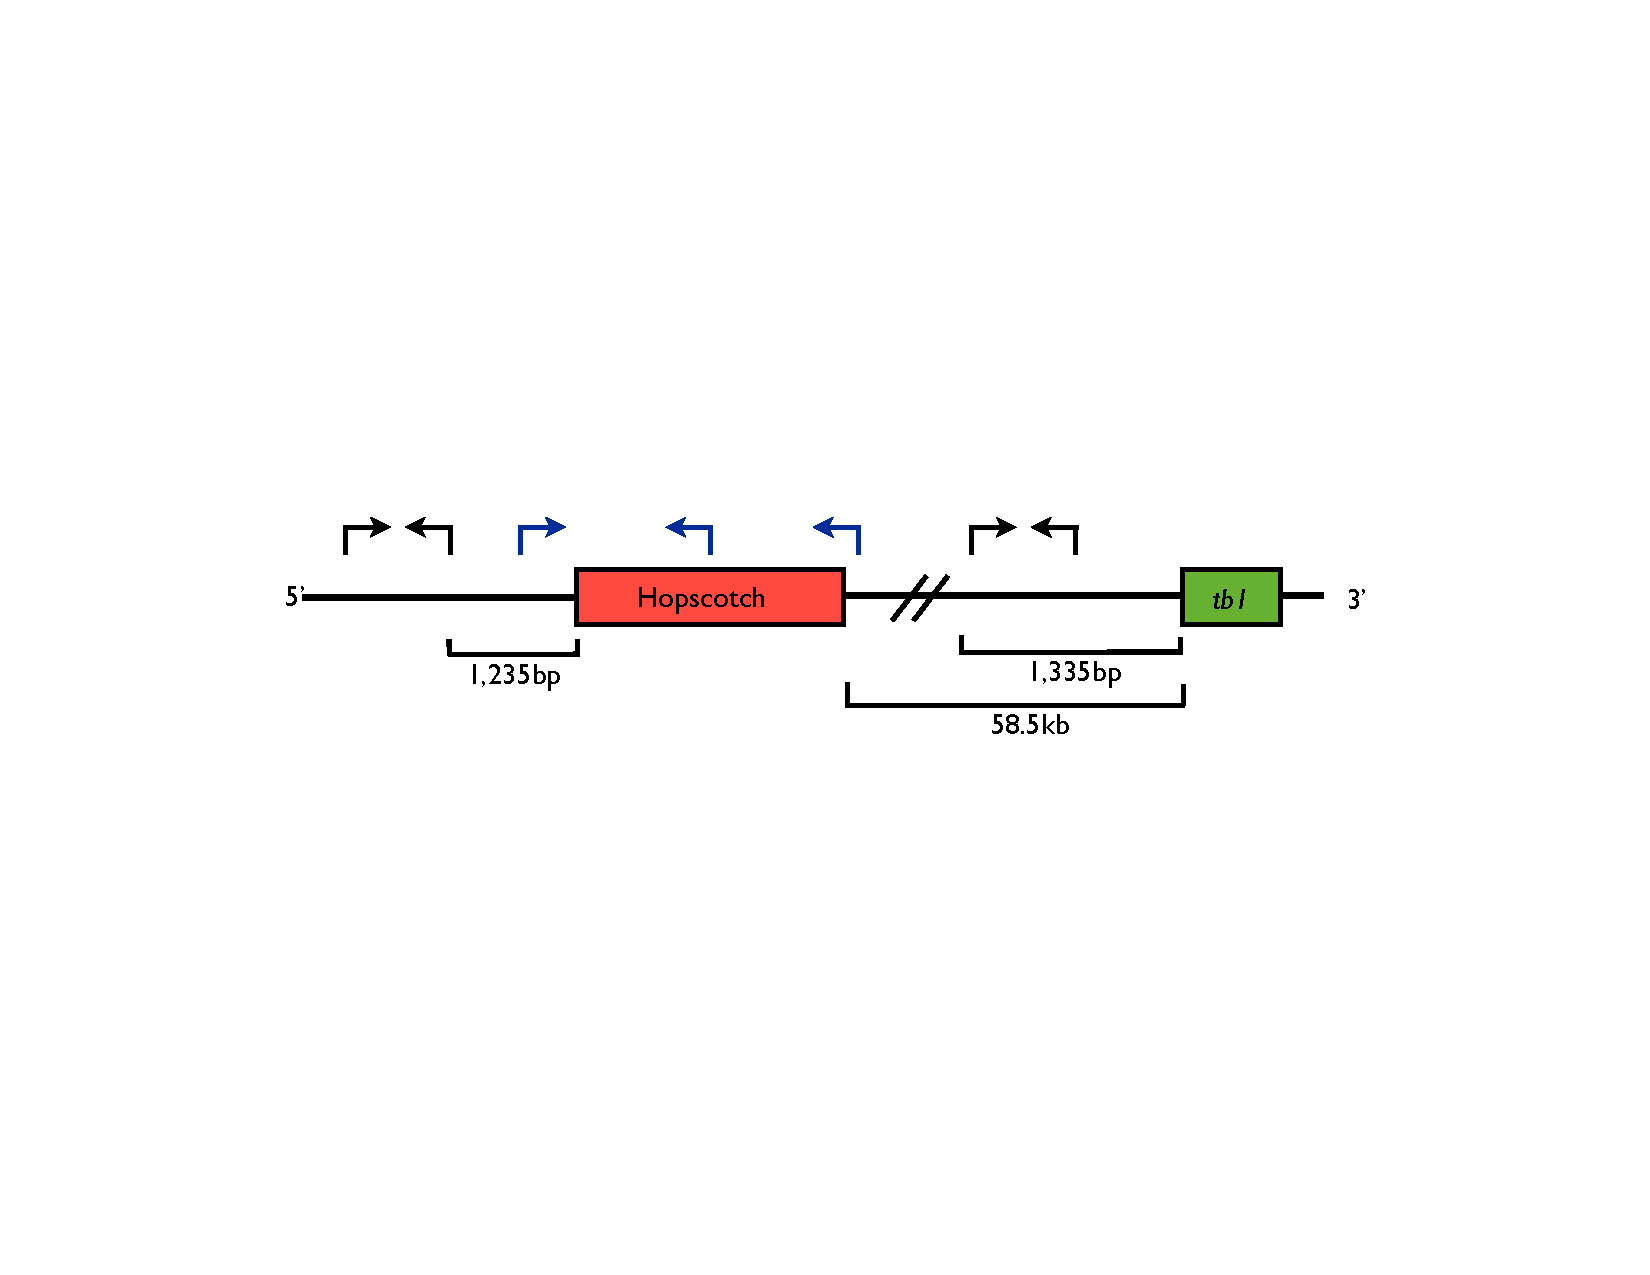
\includegraphics[width=140mm]{FigS1LocusCartoon.pdf}
   \caption{Representation of the upstream regulatory region of \emph{tb1}, showing the \emph{tb1} coding region (green) and the \emph{Hopscotch} insertion (red). Arrows show the location of primer sets; in black, primers used for amplification and sequencing (Sequenced region 1; within the 5' UTR, and sequenced region 2; 66,169 bp upstream from the tb1 ORF); in blue, primers used to genotype the \emph{Hopscotch} insertion.}
\label{FigS1Locus}
  \end{center}
\end{figure*}
%-------------------------------------------------------------------

% Figure S2. Gel image
%-------------------------------------------------------------------
\begin{figure*}[!t]
  \begin{center}
   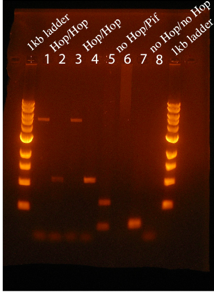
\includegraphics[width=150mm]{FigS2Gel.png}
   \caption{Agarose gel image of amplification products using our primer sets. Genotypes are indicated at the top of the gel.} 
\label{FigS2Gel}
  \end{center}
\end{figure*}
%-------------------------------------------------------------------

% Figure S3. NJ Trees
%-------------------------------------------------------------------
\begin{figure*}[!t]
  \begin{center}
   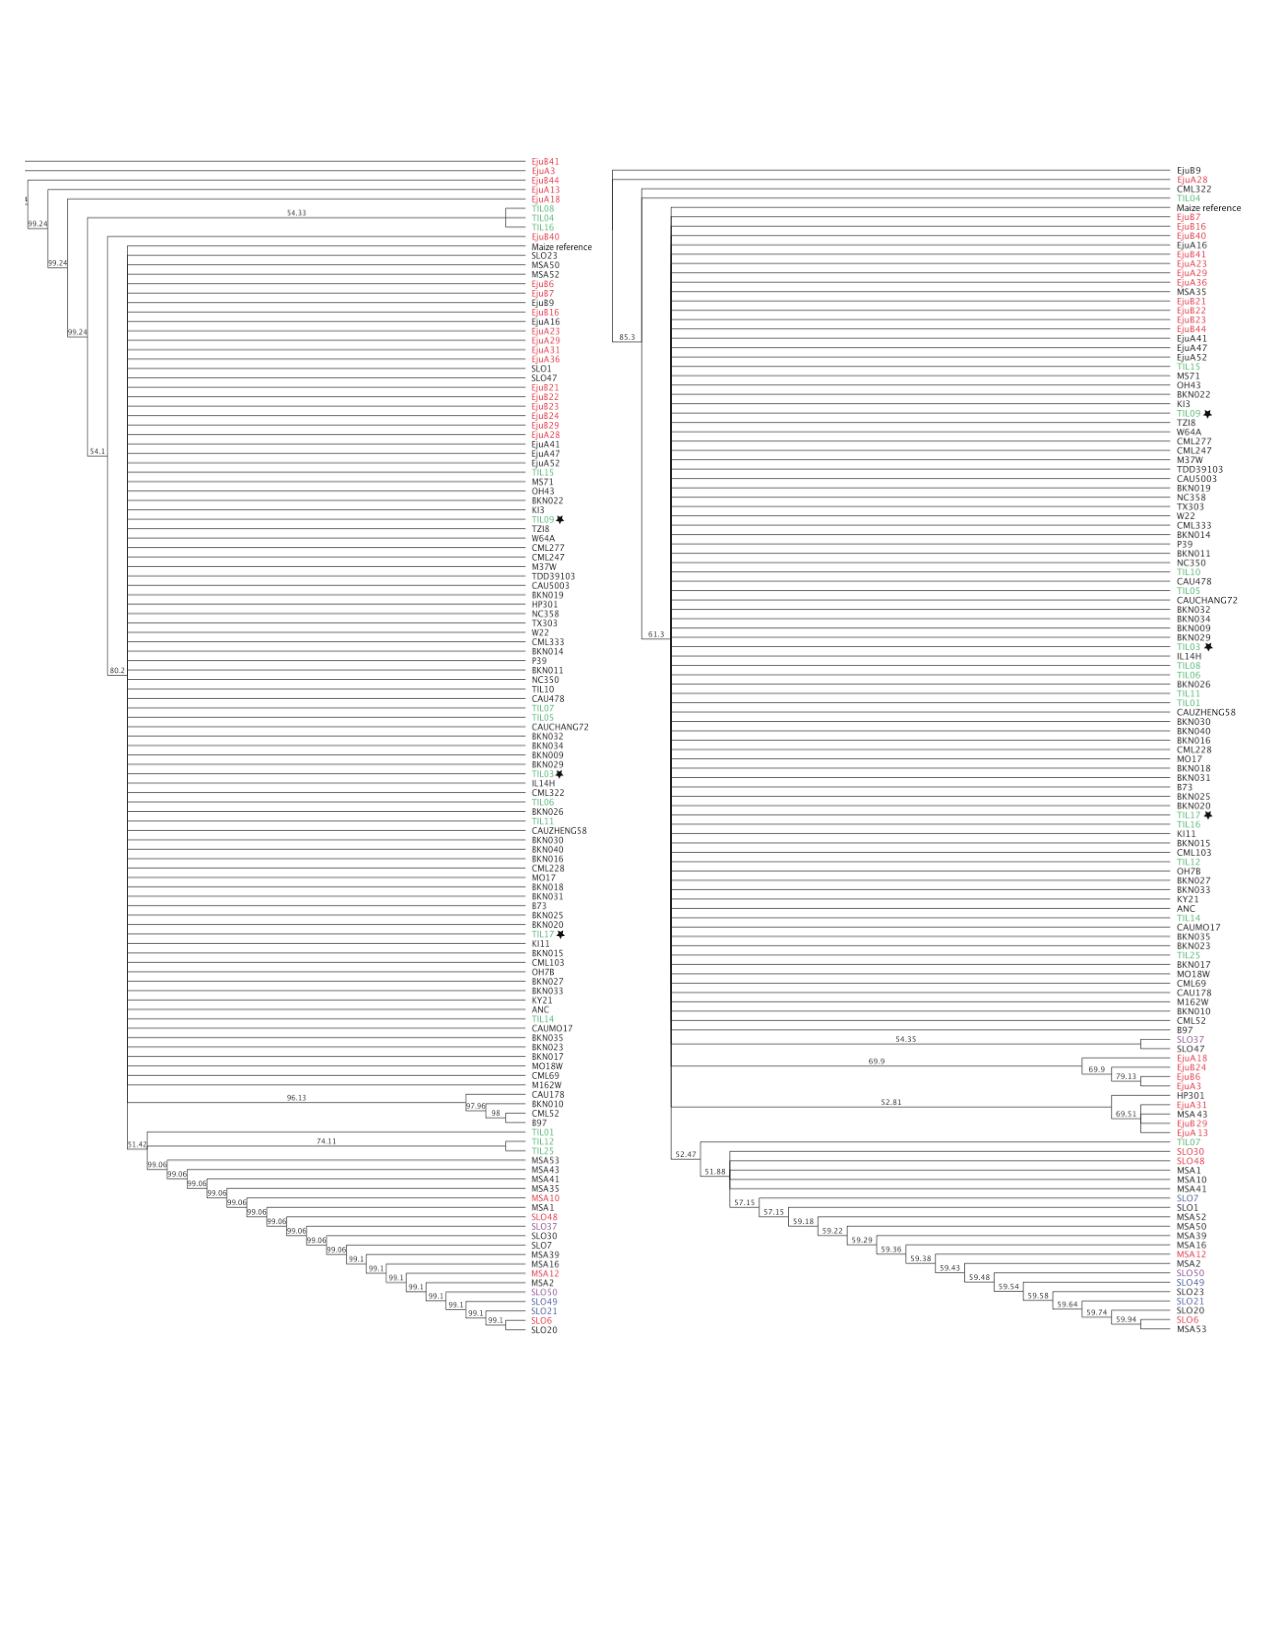
\includegraphics[width=150mm]{FigS3NJtrees.pdf}
    \caption{Neighbor-Joining tree of the sequenced region in the 5? UTR (right; sequenced region 1) and the 66,169 bp upstream region (left; sequenced region 2) of \emph{tb1}. Individuals with genotype data are colored: Homozygous for the teosinte (no \emph{Hopscotch}) allele (red), homozygous for the maize (\emph{Hopscotch}) allele (blue), heterozygotes (purple). TILs (teosinte inbred lines) are colored in green, with stars indicating the 3 TILs known to have the \emph{Hopscotch} insertion. Black indicates individuals not genotyped for the \emph{Hopscotch} insertion.} 
\label{FigS3NJ}
  \end{center}
\end{figure*}
%-------------------------------------------------------------------

% Table S1. Parv and mex samples
\begin{table}[htbp]
  \centering
  \caption{Accessions of \emph{Zea mays} ssp. \emph{mexicana} (RIMME) and \emph{Zea mays} ssp. \emph{parviglumis} (RIMPA) sampled. RIHY is a \emph{Z. mays} ssp. \emph{parviglumis} and \emph{Zea mays} ssp. \emph{mays} hybrid. }
    \begin{tabular}{rrrrrr}
%    \toprule
    Accession & USDA Accession ID & Locality & Number alleles sampled & \emph{Hopscotch} Frequency & No \emph{Hopscotch} Frequency \\
 %   \midrule
    RIHY0009 & N/A   & N/A   & 2     & 0.5   & 0.5 \\
    RIMME0006 & 566673 & Durango, Mexico & 2     & 0     & 1 \\
    RIMME0007 & 566680 & Guanajuato, Mexico & 2     & 0     & 1 \\
    RIMME0008 & 566681 & Michoacan, Mexico & 2     & 0     & 1 \\
    RIMME0009 & 566682 & Distrito Federal, Mexico & 2     & 0     & 1 \\
    RIMME0011 & 566685 & Mexico, Mexico & 2     & 0     & 1 \\
    RIMME0014 & 714151 & Breeders line; Puga: 11066 & 6     & 0     & 1 \\
    RIMME0017 & 699874 & Ayotlan, Mexico & 8     & 0     & 1 \\
    RIMME0021 & N/A   & El Porvenir, Mexico & 69    & 0.173913043 & 0.826086957 \\
    RIMME0026 & N/A   & Opopeo, Mexico & 42    & 0.071428571 & 0.928571429 \\
    RIMME0028 & N/A   & Puruandiro, Mexico & 28    & 0.035714286 & 0.964285714 \\
    RIMME0029 & N/A   & Ixtlan, Mexico & 35    & 0     & 1 \\
    RIMME0030 & N/A   & San Pedro, Mexico & 27    & 0     & 1 \\
    RIMME0031 & N/A   & Tenango del Aire, Mexico & 25    & 0.08  & 0.92 \\
    RIMME0032 & N/A   & Nabogame, Mexico & 24    & 0     & 1 \\
    RIMME0033 & N/A   & Puerta Encantada, Mexico & 25    & 0     & 1 \\
    RIMME0034 & N/A   & Santa Clara, Mexico & 23    & 0     & 1 \\
    RIMME0035 & N/A   & Xochimilco, Mexico & 25    & 0     & 1 \\
    RIMPA0001 & 87168 & El Salado, Mexico & 4     & 0     & 1 \\
    RIMPA0003 & 87171 & Mazatlan, Mexico & 8     & 0.125 & 0.875 \\
    RIMPA0017 & 87200 & N/A   & 4     & 0     & 1 \\
    RIMPA0019 & 87213 & El Salado, Mexico & 2     & 0.5   & 0.5 \\
    RIMPA0029 & 87244 & N/A   & 2     & 0.5   & 0.5 \\
    RIMPA0031 & 87249 & N/A   & 2     & 0.5   & 0.5 \\
    RIMPA0035 & 87288 & Jalisco, Mexico & 4     & 0     & 1 \\
    RIMPA0040 & 288185 & Mexico, Mexico & 4     & 0     & 1 \\
    RIMPA0042 & 288187 & Guerrero, Mexico & 4     & 0.25  & 0.75 \\
    RIMPA0043 & 288188 & Guerrero, Mexico & 4     & 0     & 1 \\
    RIMPA0045 & 288193 & Guerrero, Mexico & 4     & 0     & 1 \\
    RIMPA0055 & 714152 & Breeders line & 2     & 0     & 1 \\
    RIMPA0056 & 714153 & Breeders line & 2     & 0.5   & 0.5 \\
    RIMPA0057 & 714154 & Breeders line & 2     & 0.5   & 0.5 \\
    RIMPA0058 & N/A   & N/A   & 4     & 0.5   & 0.5 \\
    RIMPA0059 & N/A   & N/A   & 4     & 1     & 0 \\
    RIMPA0060 & 714157 & Breeders line: CIMMYT 11355 & 2     & 0     & 1 \\
    RIMPA0061 & 714158 & Breeders line: USDA PI566686 & 4     & 0.5   & 0.5 \\
    RIMPA0062 & 714159 & Breeders line & 4     & 0.5   & 0.5 \\
    RIMPA0063 & 714160 & Breeders line & 4     & 0     & 1 \\
    RIMPA0064 & 714161 & Breeders line & 3     & 0     & 1 \\
    RIMPA0065 & 714162 & Breeders line & 4     & 0.25  & 0.75 \\
    RIMPA0068 & 699861 & Jalisco, Mexico & 16    & 0     & 1 \\
    RIMPA0069 & 699862 & Ixtlan, Mexico & 14    & 0.142857143 & 0.857142857 \\
    RIMPA0070 & 699863 & Benito Jaurez, Mexico & 16    & 0     & 1 \\
    RIMPA0071 & 699864 & Tuzantla, Mexico & 28    & 0     & 1 \\
    RIMPA0072 & 699865 & Tiquicheo, Mexico & 16    & 0     & 1 \\
    RIMPA0073 & 699866 & Tiquicheo, Mexico & 16    & 0.125 & 0.875 \\
    RIMPA0074 & 699867 & Huetamo, Mexico & 12    & 0     & 1 \\
    RIMPA0075 & 699868 & Huetamo, Mexico & 2     & 0     & 1 \\
    RIMPA0076 & 699869 & Huetamo, Mexico & 4     & 0     & 1 \\
    RIMPA0077 & 699870 & Caracuaro, Mexico & 2     & 0     & 1 \\
    RIMPA0078 & 699871 & Caracuaro, Mexico & 2     & 0.5   & 0.5 \\
    RIMPA0079 & 699872 & Villa Madero, Mexico & 14    & 0     & 1 \\
    RIMPA0080 & 699873 & Guachinango, Mexico & 12    & 0     & 1 \\
    RIMPA0081 & 699875 & Ameca, Mexico & 16    & 0     & 1 \\
    RIMPA0083 & 699877 & Tepoztlan, Mexico & 14    & 0     & 1 \\
    RIMPA0084 & 699878 & Tepoztlan, Mexico & 16    & 0     & 1 \\
    RIMPA0085 & 699879 & Miahuatlan, Mexico & 16    & 0     & 1 \\
    RIMPA0086 & 699880 & Miahuatlan, Mexico & 16    & 0.0625 & 0.9375 \\
    RIMPA0087 & 699881 & Tecoanapa, Mexico & 24    & 0     & 1 \\
    RIMPA0089 & 699883 & Guerrero, Mexico & 12    & 0     & 1 \\
    RIMPA0090 & 699884 & Guerrero, Mexico & 10    & 0     & 1 \\
    RIMPA0091 & 699885 & Guerrero, Mexico & 16    & 0     & 1 \\
    RIMPA0092 & 699886 & Guerrero, Mexico & 10    & 0     & 1 \\
    RIMPA0093 & 699887 & Guerrero, Mexico & 26    & 0.076923077 & 0.923076923 \\
    RIMPA0094 & 699888 & Guerrero, Mexico & 2     & 0     & 1 \\
    RIMPA0095 & 699889 & Guerrero, Mexico & 4     & 0     & 1 \\
    RIMPA0096 & 699890 & Guerrero, Mexico & 26    & 0.038461538 & 0.961538462 \\
    RIMPA0097 & 699891 & Guerrero, Mexico & 6     & 0     & 1 \\
    RIMPA0098 & 699892 & Guerrero, Mexico & 4     & 0     & 1 \\
    RIMPA0099 & 699893 & Guerrero, Mexico & 4     & 0     & 1 \\
    RIMPA0100 & 699894 & Guerrero, Mexico & 6     & 0     & 1 \\
    RIMPA0101 & 699895 & Guerrero, Mexico & 2     & 0     & 1 \\
    RIMPA0103 & 699897 & Guerrero, Mexico & 2     & 0     & 1 \\
    RIMPA0104 & 699898 & Guerrero, Mexico & 22    & 0.090909091 & 0.909090909 \\
    RIMPA0105 & 699899 & Guerrero, Mexico & 6     & 0     & 1 \\
    RIMPA0106 & 699900 & Guerrero, Mexico & 6     & 0.333333333 & 0.666666667 \\
    RIMPA0107 & 699901 & Guerrero, Mexico & 4     & 0     & 1 \\
    RIMPA0108 & 699902 & Guerrero, Mexico & 6     & 0     & 1 \\
    RIMPA0109 & 699903 & Michoacan, Mexico & 4     & 0.25  & 0.75 \\
    RIMPA0110 & 699904 & Michoacan, Mexico & 2     & 0     & 1 \\
    RIMPA0111 & 699905 & Michoacan, Mexico & 4     & 0     & 1 \\
    RIMPA0112 & 699906 & Michoacan, Mexico & 4     & 0.25  & 0.75 \\
    RIMPA0114 & 699908 & Michoacan, Mexico & 6     & 0.166666667 & 0.833333333 \\
    RIMPA0116 & 699910 & Mexico, Mexico & 2     & 0     & 1 \\
    RIMPA0117 & 699911 & Mexico, Mexico & 4     & 0     & 1 \\
    RIMPA0118 & 699912 & Mexico, Mexico & 6     & 0.166666667 & 0.833333333 \\
    RIMPA0119 & 699913 & Mexico, Mexico & 2     & 0     & 1 \\
    RIMPA0120 & 699914 & Mexico, Mexico & 1     & 1     & 0 \\
    RIMPA0121 & 699915 & Mexico, Mexico & 2     & 0     & 1 \\
    RIMPA0128 & 699922 & Mexico, Mexico & 2     & 0.5   & 0.5 \\
    RIMPA0129 & 699923 & Michoacan, Mexico & 2     & 0.5   & 0.5 \\
    RIMPA0135 & 699929 & Nayarit, Mexico & 24    & 0     & 1 \\
    RIMPA0138 & 699932 & Jalisco, Mexico & 2     & 0.5   & 0.5 \\
    RIMPA0139 & 699933 & Jalisco, Mexico & 1     & 1     & 0 \\
    RIMPA0142 & 699936 & Colima, Mexico & 18    & 0.444444444 & 0.555555556 \\
    RIMPA0144 & 699938 & Jalisco, Mexico & 2     & 1     & 0 \\
    RIMPA0145 & 699939 & Michoacan, Mexico & 1     & 1     & 0 \\
    RIMPA0147 & 699941 & Jalisco, Mexico & 1     & 1     & 0 \\
    RIMPA0155 & N/A   & Jalisco, Mexico & 73    & 0.01369863 & 0.98630137 \\
    RIMPA0156 & N/A   & Jalisco, Mexico & 20    & 0     & 1 \\
    RIMPA0157 & N/A   & Jalisco, Mexico & 58    & 0.344827586 & 0.655172414 \\
    RIMPA0158 & N/A   & Jalisco, Mexico & 64    & 0.53125 & 0.46875 \\
    RIMPA0159 & N/A   & Jalisco, Mexico & 26    & 0     & 1 \\
    RIMPA0162 & 21785 & N/A   & 4     & 0     & 1 \\
 %   \bottomrule
    \end{tabular}
  \label{TableS1}
\end{table}

% Table S2. Mays sampling
\begin{table}[htbp]
  \centering
 \caption{\emph{Zea mays} ssp. \emph{mays} (RIMMA) sampled for genotyping}
    \begin{tabular}{ccc}
 %   \toprule
    Accession & Number of alleles sampled & \emph{Hopscotch} Frequency \\
 %   \midrule
    RIMMA0066 & 2     & 1 \\
    RIMMA0075 & 2     & 1 \\
    RIMMA0077 & 2     & 1 \\
    RIMMA0079 & 2     & 1 \\
    RIMMA0081 & 2     & 1 \\
    RIMMA0084 & 2     & 1 \\
    RIMMA0086 & 2     & 1 \\
    RIMMA0088 & 2     & 1 \\
    RIMMA0089 & 2     & 1 \\
    RIMMA0090 & 2     & 1 \\
    RIMMA0092 & 4     & 1 \\
    RIMMA0094 & 4     & 1 \\
    RIMMA0097 & 2     & 1 \\
    RIMMA0099 & 2     & 1 \\
    RIMMA0100 & 2     & 1 \\
    RIMMA0101 & 2     & 1 \\
    RIMMA0104 & 2     & 1 \\
    RIMMA0108 & 2     & 1 \\
    RIMMA0111 & 6     & 1 \\
    RIMMA0115 & 2     & 1 \\
    RIMMA0117 & 2     & 1 \\
    RIMMA0130 & 2     & 1 \\
    RIMMA0133 & 2     & 1 \\
    RIMMA0134 & 2     & 1 \\
    RIMMA0135 & 2     & 1 \\
    RIMMA0142 & 2     & 0.5 \\
    RIMMA0143 & 4     & 1 \\
    RIMMA0146 & 4     & 1 \\
    RIMMA0149 & 2     & 1 \\
    RIMMA0152 & 2     & 1 \\
    RIMMA0153 & 2     & 1 \\
    RIMMA0154 & 2     & 1 \\
    RIMMA0155 & 2     & 1 \\
    RIMMA0156 & 2     & 1 \\
    RIMMA0157 & 2     & 1 \\
    RIMMA0158 & 2     & 1 \\
    RIMMA0159 & 2     & 1 \\
    RIMMA0160 & 2     & 1 \\
    RIMMA0162 & 2     & 1 \\
    RIMMA0166 & 2     & 1 \\
    RIMMA0167 & 2     & 1 \\
    RIMMA0168 & 2     & 1 \\
    RIMMA0169 & 2     & 1 \\
    RIMMA0172 & 2     & 1 \\
    RIMMA0174 & 4     & 1 \\
    RIMMA0177 & 2     & 1 \\
    RIMMA0178 & 2     & 1 \\
    RIMMA0179 & 2     & 1 \\
    RIMMA0181 & 2     & 1 \\
    RIMMA0183 & 2     & 1 \\
    RIMMA0184 & 2     & 1 \\
    RIMMA0186 & 2     & 1 \\
    RIMMA0187 & 1     & 1 \\
    RIMMA0188 & 2     & 1 \\
    RIMMA0195 & 2     & 1 \\
    RIMMA0196 & 2     & 1 \\
    RIMMA0197 & 2     & 1 \\
    RIMMA0198 & 2     & 1 \\
    RIMMA0199 & 2     & 1 \\
    RIMMA0200 & 2     & 1 \\
    RIMMA0202 & 2     & 1 \\
    RIMMA0203 & 2     & 1 \\
    RIMMA0206 & 2     & 1 \\
    RIMMA0208 & 2     & 1 \\
    RIMMA0209 & 2     & 1 \\
    RIMMA0210 & 2     & 1 \\
    RIMMA0212 & 2     & 1 \\
    RIMMA0213 & 2     & 1 \\
    RIMMA0214 & 2     & 1 \\
    RIMMA0217 & 2     & 1 \\
    RIMMA0218 & 2     & 1 \\
    RIMMA0220 & 2     & 1 \\
    RIMMA0221 & 2     & 1 \\
    RIMMA0222 & 2     & 1 \\
    RIMMA0223 & 2     & 1 \\
    RIMMA0226 & 2     & 1 \\
    RIMMA0227 & 2     & 1 \\
    RIMMA0228 & 2     & 1 \\
    RIMMA0229 & 2     & 1 \\
    RIMMA0230 & 2     & 1 \\
    RIMMA0232 & 2     & 1 \\
    RIMMA0233 & 2     & 1 \\
    RIMMA0235 & 2     & 0.5 \\
    RIMMA0242 & 2     & 1 \\
    RIMMA0243 & 2     & 1 \\
    RIMMA0247 & 4     & 1 \\
    RIMMA0248 & 2     & 1 \\
    RIMMA0249 & 2     & 1 \\
    RIMMA0252 & 2     & 1 \\
    RIMMA0253 & 2     & 1 \\
    RIMMA0254 & 2     & 1 \\
    RIMMA0256 & 2     & 1 \\
    RIMMA0257 & 2     & 1 \\
    RIMMA0258 & 2     & 1 \\
    RIMMA0259 & 2     & 1 \\
    RIMMA0260 & 2     & 1 \\
    RIMMA0262 & 2     & 1 \\
    RIMMA0263 & 2     & 1 \\
    RIMMA0264 & 2     & 1 \\
    RIMMA0265 & 2     & 1 \\
    RIMMA0268 & 2     & 1 \\
    RIMMA0269 & 2     & 1 \\
    RIMMA0270 & 2     & 1 \\
    RIMMA0272 & 2     & 1 \\
    RIMMA0275 & 2     & 1 \\
    RIMMA0276 & 2     & 1 \\
    RIMMA0277 & 2     & 1 \\
    RIMMA0279 & 2     & 1 \\
    RIMMA0280 & 2     & 1 \\
    RIMMA0283 & 2     & 1 \\
    RIMMA0285 & 2     & 1 \\
    RIMMA0288 & 2     & 1 \\
    RIMMA0290 & 2     & 1 \\
    RIMMA0291 & 2     & 1 \\
    RIMMA0292 & 2     & 1 \\
    RIMMA0293 & 2     & 1 \\
    RIMMA0298 & 2     & 1 \\
    RIMMA0302 & 2     & 1 \\
    RIMMA0305 & 2     & 1 \\
    RIMMA0310 & 2     & 1 \\
    RIMMA0312 & 2     & 1 \\
    RIMMA0320 & 2     & 1 \\
    RIMMA0322 & 2     & 1 \\
    RIMMA0324 & 2     & 1 \\
    RIMMA0334 & 2     & 1 \\
    RIMMA0336 & 2     & 1 \\
    RIMMA0337 & 2     & 1 \\
    RIMMA0338 & 2     & 1 \\
    RIMMA0339 & 2     & 1 \\
    RIMMA0340 & 2     & 1 \\
    RIMMA0341 & 2     & 1 \\
    RIMMA0342 & 2     & 1 \\
    RIMMA0344 & 2     & 1 \\
    RIMMA0346 & 2     & 1 \\
    RIMMA0347 & 2     & 1 \\
    RIMMA0350 & 2     & 1 \\
    RIMMA0351 & 2     & 1 \\
    RIMMA0352 & 2     & 1 \\
    RIMMA0357 & 2     & 1 \\
    RIMMA0360 & 18    & 1 \\
    RIMMA0362 & 8     & 1 \\
    RIMMA0363 & 16    & 1 \\
    RIMMA0370 & 17    & 1 \\
    RIMMA0372 & 24    & 1 \\
    RIMMA0373 & 22    & 1 \\
    RIMMA0408 & 2     & 1 \\
    RIMMA0411 & 1     & 1 \\
    RIMMA0413 & 1     & 1 \\
    RIMMA0414 & 1     & 1 \\
    RIMMA0424 & 8     & 0.9 \\
    RIMMA0432 & 1     & 1 \\
    RIMMA0434 & 2     & 0.5 \\
    RIMMA0435 & 1     & 1 \\
    RIMMA0442 & 2     & 1 \\
    RIMMA0443 & 2     & 1 \\
    RIMMA0444 & 2     & 1 \\
    RIMMA0445 & 2     & 1 \\
    RIMMA0446 & 2     & 1 \\
    RIMMA0447 & 2     & 1 \\
    RIMMA0448 & 2     & 1 \\
    RIMMA0449 & 2     & 1 \\
    RIMMA0450 & 2     & 1 \\
    RIMMA0451 & 2     & 1 \\
    RIMMA0452 & 2     & 1 \\
    RIMMA0453 & 2     & 1 \\
    RIMMA0454 & 2     & 1 \\
    RIMMA0455 & 2     & 1 \\
    RIMMA0456 & 2     & 1 \\
    RIMMA0457 & 2     & 1 \\
    RIMMA0458 & 2     & 1 \\
    RIMMA0459 & 2     & 1 \\
    RIMMA0483 & 2     & 1 \\
    RIMMA0490 & 2     & 1 \\
    RIMMA0515 & 2     & 1 \\
    RIMMA0537 & 2     & 1 \\
    RIMMA0550 & 2     & 1 \\
    RIMMA0553 & 2     & 1 \\
    RIMMA0559 & 2     & 1 \\
    RIMMA0561 & 2     & 1 \\
    RIMMA0562 & 2     & 1 \\
    RIMMA0571 & 2     & 1 \\
    RIMMA0572 & 2     & 1 \\
    RIMMA0577 & 2     & 1 \\
    RIMMA0579 & 2     & 1 \\
    RIMMA0590 & 2     & 1 \\
    RIMMA0591 & 2     & 1 \\
    RIMMA0592 & 2     & 1 \\
    RIMMA0593 & 2     & 1 \\
    RIMMA0594 & 2     & 1 \\
    RIMMA0595 & 2     & 1 \\
    RIMMA0596 & 2     & 1 \\
    RIMMA0597 & 2     & 1 \\
    RIMMA0598 & 2     & 1 \\
    RIMMA0599 & 2     & 1 \\
    RIMMA0600 & 2     & 1 \\
    RIMMA0601 & 2     & 1 \\
    RIMMA0602 & 2     & 1 \\
    RIMMA0603 & 2     & 1 \\
    RIMMA0604 & 2     & 1 \\
    RIMMA0605 & 2     & 1 \\
    RIMMA0606 & 2     & 1 \\
    RIMMA0607 & 2     & 1 \\
    RIMMA0608 & 2     & 1 \\
    RIMMA0609 & 2     & 1 \\
    RIMMA0610 & 2     & 1 \\
    RIMMA0611 & 2     & 1 \\
    RIMMA0612 & 2     & 1 \\
    RIMMA0613 & 2     & 1 \\
    RIMMA0622 & 2     & 0.5 \\
    RIMMA0624 & 1     & 1 \\
    RIMMA0629 & 2     & 0.5 \\
    RIMMA0631 & 2     & 0.5 \\
    RIMMA0659 & 2     & 1 \\
    RIMMA0660 & 2     & 1 \\
    RIMMA0678 & 1     & 1 \\
    RIMMA0681 & 2     & 1 \\
    RIMMA0683 & 2     & 1 \\
    RIMMA0684 & 2     & 1 \\
    RIMMA0685 & 4     & 1 \\
    RIMMA0693 & 2     & 1 \\
    RIMMA0694 & 2     & 1 \\
    RIMMA0695 & 1     & 1 \\
    RIMMA0699 & 2     & 1 \\
    RIMMA0704 & 2     & 1 \\
    RIMMA0706 & 2     & 1 \\
    RIMMA0711 & 1     & 1 \\
    RIMMA0713 & 2     & 1 \\
    RIMMA0715 & 2     & 1 \\
    RIMMA0717 & 2     & 1 \\
    RIMMA0718 & 2     & 1 \\
    RIMMA0723 & 2     & 1 \\
    RIMMA0724 & 2     & 1 \\
    RIMMA0725 & 1     & 1 \\
    RIMMA0728 & 1     & 1 \\
    RIMMA0732 & 2     & 1 \\
    RIMMA0734 & 2     & 1 \\
    RIMMA0738 & 2     & 1 \\
    RIMMA0739 & 2     & 1 \\
    RIMMA0744 & 2     & 1 \\
    RIMMA0747 & 1     & 1 \\
    RIMMA0748 & 2     & 1 \\
    RIMMA0749 & 2     & 1 \\
    RIMMA0750 & 2     & 0.5 \\
    RIMMA0751 & 1     & 1 \\
    RIMMA0752 & 1     & 1 \\
    RIMMA0753 & 2     & 1 \\
    RIMMA0755 & 2     & 1 \\
    \bottomrule
    \end{tabular}
  \label{TableS2Mays}
\end{table}


% Table S3. PCs for BayEnv
\begin{table}[htbp]
  \centering
  \caption{Variables and rotations used for the 6 principal components used for BayEnv calculations and their corresponding Bayes Factors. Modified from \citet{Pyhajarvi2013}.}
    \begin{tabular}{rrrrrrrrrrrr}
    \toprule
    \textbf{PC1} & \textbf{} & \textbf{PC2} & \textbf{} & \textbf{PC3} & \textbf{} & \textbf{PC4} & \textbf{} & \textbf{PC5} & \textbf{} & \textbf{PC6} & \textbf{} \\
    \midrule
    \textbf{Var} & \textbf{Rot} & \textbf{Var} & \textbf{Rot} & \textbf{Var} & \textbf{Rot} & \textbf{Var} & \textbf{Rot} & \textbf{Var} & \textbf{Rot} & \textbf{Var} & \textbf{Rot} \\
    bio1  & 0.146 & bio4  & 0.244 & prec7 & 0.287 & ts\_clay & 0.41  & bio2  & 0.38  & bio2  & 0.412 \\
    tmean11 & 0.146 & bio3  & 0.241 & prec8 & 0.276 & v\_mod & 0.359 & sq4   & 0.328 & x\_mod & 0.365 \\
    tmean12 & 0.145 & bio7  & 0.241 & prec11 & 0.262 & ts\_sand & 0.329 & ts\_loam & 0.289 & sq7   & 0.332 \\
    bio11 & 0.145 & prec6 & 0.237 & bio13 & 0.247 & bio15 & 0.272 & ts\_sand & 0.266 & bio7  & 0.312 \\
    tmax12 & 0.145 & sq7   & 0.218 & prec1 & 0.246 & prec4 & 0.259 & sq7   & 0.231 & v\_mod & 0.307 \\
    tmin5 & 0.145 & prec9 & 0.217 & bio16 & 0.242 & x\_mod & 0.244 & bio18 & 0.213 & prec11 & 0.23 \\
    tmean1 & 0.145 & sq3   & 0.207 & prec12 & 0.24  & prec3 & 0.226 & bio13 & 0.207 & bio18 & 0.22 \\
    tmean2 & 0.145 & prec12 & 0.207 & bio19 & 0.238 & sq3   & 0.21  & prec11 & 0.183 & sq3   & 0.176 \\
    tmin4 & 0.145 & bio12 & 0.204 & bio12 & 0.231 & prec5 & 0.21  & bio7  & 0.17  & sq4   & 0.153 \\
    tmax1 & 0.145 & bio19 & 0.196 & prec2 & 0.222 & prec7 & 0.19  & bio16 & 0.163 & ts\_sand & 0.153 \\
    tmean4 & 0.145 & prec2 & 0.188 & bio18 & 0.221 & sq4   & 0.186 & bio4  & 0.157 & bio4  & 0.148 \\
    tmin11 & 0.144 & prec1 & 0.185 & sq4   & 0.2   & bio3  & 0.185 & bio12 & 0.156 & prec7 & 0.139 \\
    tmax11 & 0.144 & prec10 & 0.184 & prec9 & 0.18  & bio18 & 0.178 & bio3  & 0.155 & tmax3 & 0.127 \\
    tmin12 & 0.144 & bio16 & 0.183 & prec10 & 0.171 & sq7   & 0.132 & prec6 & 0.154 & tmax4 & 0.126 \\
    tmin2 & 0.144 & prec8 & 0.17  & prec5 & 0.161 & bio14 & 0.116 & x\_mod & 0.152 & bio5  & 0.118 \\
    tmean5 & 0.144 & prec5 & 0.165 & prec4 & 0.154 & bio13 & 0.099 & prec9 & 0.144 & tmax5 & 0.115 \\
    tmean10 & 0.144 & bio14 & 0.158 & sq3   & 0.147 & bio16 & 0.095 & prec8 & 0.143 & bio3  & 0.107 \\
    bio6  & 0.144 & bio13 & 0.151 & bio2  & 0.143 & prec8 & 0.09  & v\_mod & 0.142 & ts\_loam & 0.095 \\
    tmax2 & 0.144 & bio17 & 0.149 & bio17 & 0.129 & bio7  & 0.077 & bio15 & 0.136 & ts\_clay & 0.078 \\
    tmean3 & 0.144 & prec3 & 0.144 & ts\_loam & 0.127 & bio4  & 0.075 & prec7 & 0.112 & tmin9 & 0.072 \\
    tmin1 & 0.143 & ts\_clay & 0.141 & v\_mod & 0.123 & bio2  & 0.074 & prec4 & 0.108 & tmin8 & 0.071 \\
    tmin10 & 0.143 & bio2  & 0.129 & prec3 & 0.113 & prec2 & 0.074 & bio14 & 0.096 & prec9 & 0.07 \\
    Altitude & 0.143 & prec7 & 0.108 & x\_mod & 0.111 & bio19 & 0.068 & tmax7 & 0.093 & tmin10 & 0.069 \\
    bio9  & 0.143 & tmax6 & 0.107 & bio14 & 0.099 & prec12 & 0.056 & tmax8 & 0.092 & tmin12 & 0.069 \\
    tmin3 & 0.143 & x\_mod & 0.106 & bio4  & 0.07  & ts\_loam & 0.053 & prec1 & 0.091 & tmin7 & 0.066 \\
    bio10 & 0.142 & bio15 & 0.098 & tmax3 & 0.067 & tmax12 & 0.047 & prec2 & 0.086 & tmean4 & 0.066 \\
    tmax10 & 0.142 & ts\_loam & 0.088 & ts\_clay & 0.065 & bio17 & 0.047 & tmin11 & 0.086 & tmax2 & 0.066 \\
    tmax3 & 0.142 & tmean6 & 0.085 & bio15 & 0.056 & bio9  & 0.043 & prec5 & 0.082 & tmax6 & 0.064 \\
    tmax4 & 0.142 & tmin7 & 0.082 & tmax2 & 0.055 & tmax8 & 0.042 & bio17 & 0.082 & tmean3 & 0.064 \\
    tmin6 & 0.142 & bio5  & 0.082 & tmean3 & 0.052 & tmax1 & 0.041 & tmin12 & 0.08  & bio9  & 0.058 \\
    tmean9 & 0.141 & tmean7 & 0.081 & ts\_sand & 0.05  & tmax5 & 0.039 & prec3 & 0.078 & tmin11 & 0.058 \\
    tmin9 & 0.141 & prec4 & 0.08  & prec6 & 0.048 & tmax7 & 0.039 & tmax9 & 0.078 & prec3 & 0.056 \\
    tmean8 & 0.141 & tmax7 & 0.079 & sq7   & 0.048 & prec10 & 0.038 & tmin1 & 0.077 & tmean5 & 0.056 \\
    bio8  & 0.14  & bio8  & 0.079 & tmin7 & 0.046 & Altitude & 0.037 & tmin10 & 0.074 & bio10 & 0.051 \\
    tmean6 & 0.14  & tmax9 & 0.077 & bio3  & 0.044 & tmax10 & 0.035 & bio6  & 0.071 & bio15 & 0.047 \\
    tmean7 & 0.14  & tmean8 & 0.076 & tmax4 & 0.043 & tmax2 & 0.033 & prec12 & 0.067 & tmin1 & 0.045 \\
    tmin8 & 0.14  & tmin8 & 0.076 & bio7  & 0.042 & tmax9 & 0.03  & tmin2 & 0.061 & prec12 & 0.045 \\
    tmax5 & 0.14  & tmax5 & 0.074 & tmax1 & 0.036 & tmean12 & 0.029 & tmin6 & 0.061 & bio17 & 0.045 \\
    tmax9 & 0.139 & tmax8 & 0.074 & tmin3 & 0.035 & tmax11 & 0.027 & tmax6 & 0.059 & tmean10 & 0.043 \\
    tmax8 & 0.139 & tmean9 & 0.072 & bio9  & 0.035 & tmean1 & 0.027 & tmin3 & 0.052 & prec4 & 0.043 \\
    bio5  & 0.139 & bio18 & 0.07  & tmin8 & 0.034 & bio5  & 0.026 & bio8  & 0.046 & Altitude & 0.041 \\
    tmax7 & 0.139 & v\_mod & 0.066 & tmean4 & 0.031 & tmean5 & 0.026 & tmean11 & 0.041 & bio6  & 0.039 \\
    tmin7 & 0.138 & tmin9 & 0.066 & tmean2 & 0.031 & bio11 & 0.025 & tmean1 & 0.04  & tmin6 & 0.038 \\
    tmax6 & 0.135 & bio10 & 0.065 & tmax12 & 0.03  & tmean2 & 0.022 & tmin9 & 0.04  & tmean12 & 0.035 \\
    bio17 & 0.107 & tmax10 & 0.063 & tmean7 & 0.028 & tmin6 & 0.022 & tmean12 & 0.04  & tmean9 & 0.035 \\
    bio14 & 0.095 & tmin6 & 0.061 & tmin9 & 0.023 & prec1 & 0.022 & tmax10 & 0.038 & prec5 & 0.033 \\
    prec3 & 0.094 & prec11 & 0.056 & Altitude & 0.021 & tmean7 & 0.02  & tmin5 & 0.038 & tmean8 & 0.03 \\
    bio15 & 0.092 & ts\_sand & 0.054 & tmax11 & 0.019 & tmean8 & 0.02  & bio11 & 0.037 & tmin2 & 0.03 \\
    prec4 & 0.088 & sq4   & 0.049 & tmin4 & 0.018 & tmean9 & 0.019 & tmean8 & 0.035 & tmax1 & 0.03 \\
    prec10 & 0.084 & tmin3 & 0.048 & tmax5 & 0.017 & prec11 & 0.019 & tmean7 & 0.033 & prec1 & 0.025 \\
    ts\_sand & 0.073 & tmean10 & 0.047 & tmin10 & 0.017 & tmean11 & 0.018 & tmean2 & 0.03  & bio13 & 0.024 \\
    ts\_loam & 0.072 & tmean5 & 0.044 & tmin6 & 0.017 & tmax4 & 0.016 & bio19 & 0.029 & tmean11 & 0.023 \\
    prec6 & 0.069 & tmax4 & 0.042 & tmean6 & 0.017 & tmean10 & 0.016 & bio9  & 0.027 & tmax7 & 0.023 \\
    prec9 & 0.063 & tmax11 & 0.041 & tmax6 & 0.017 & tmin5 & 0.015 & tmin7 & 0.026 & tmean7 & 0.023 \\
    prec2 & 0.063 & bio6  & 0.038 & tmin12 & 0.017 & tmean6 & 0.015 & tmin4 & 0.025 & prec10 & 0.022 \\
    bio4  & 0.06  & tmin1 & 0.038 & bio11 & 0.016 & prec6 & 0.014 & tmean5 & 0.023 & prec2 & 0.02 \\
    prec5 & 0.058 & tmin2 & 0.037 & tmin11 & 0.015 & bio6  & 0.012 & tmean3 & 0.022 & bio8  & 0.018 \\
    bio13 & 0.055 & Altitude & 0.036 & tmin1 & 0.013 & tmin1 & 0.012 & tmin8 & 0.022 & tmean2 & 0.017 \\
    x\_mod & 0.053 & tmin10 & 0.034 & tmean5 & 0.013 & tmin12 & 0.011 & tmean10 & 0.021 & bio16 & 0.016 \\
    prec1 & 0.05  & bio9  & 0.032 & tmean8 & 0.013 & tmin2 & 0.011 & tmean9 & 0.019 & tmean6 & 0.014 \\
    bio16 & 0.049 & tmean1 & 0.029 & bio6  & 0.012 & bio1  & 0.011 & tmean4 & 0.019 & bio19 & 0.012 \\
    bio7  & 0.043 & bio1  & 0.028 & tmean9 & 0.01  & tmin4 & 0.009 & ts\_clay & 0.018 & tmax11 & 0.012 \\
    bio19 & 0.042 & tmean3 & 0.026 & tmean1 & 0.01  & tmax6 & 0.008 & prec10 & 0.015 & tmax10 & 0.011 \\
    bio12 & 0.042 & tmean2 & 0.024 & bio10 & 0.01  & tmin11 & 0.007 & bio1  & 0.014 & tmax8 & 0.01 \\
    bio3  & 0.04  & bio11 & 0.022 & tmax8 & 0.009 & bio8  & 0.007 & tmax4 & 0.014 & tmean1 & 0.009 \\
    prec7 & 0.034 & tmean11 & 0.019 & tmax7 & 0.009 & bio10 & 0.007 & bio10 & 0.011 & bio14 & 0.009 \\
    prec12 & 0.033 & tmin12 & 0.019 & bio5  & 0.008 & tmin9 & 0.006 & tmax5 & 0.009 & prec8 & 0.007 \\
    bio2  & 0.033 & tmax1 & 0.017 & tmin5 & 0.008 & prec9 & 0.005 & bio5  & 0.008 & bio11 & 0.007 \\
    prec8 & 0.032 & tmean4 & 0.016 & tmin2 & 0.007 & bio12 & 0.004 & tmax11 & 0.008 & tmin5 & 0.006 \\
    sq4   & 0.026 & tmin5 & 0.013 & bio1  & 0.007 & tmax3 & 0.003 & tmax12 & 0.008 & tmax9 & 0.005 \\
    sq3   & 0.024 & tmean12 & 0.012 & tmax10 & 0.006 & tmean4 & 0.003 & tmax3 & 0.007 & bio12 & 0.004 \\
    v\_mod & 0.015 & tmax2 & 0.011 & tmean10 & 0.006 & tmin3 & 0.002 & sq3   & 0.007 & tmin3 & 0.004 \\
    ts\_clay & 0.012 & tmin4 & 0.01  & tmean12 & 0.005 & tmin7 & 0.002 & tmax2 & 0.006 & prec6 & 0.004 \\
    sq7   & 0.004 & tmax3 & 0.003 & bio8  & 0.004 & tmean3 & 0.002 & Altitude & 0.004 & tmin4 & 0.003 \\
    prec11 & 0.004 & tmax12 & 0.002 & tmax9 & 0.003 & tmin10 & 0.002 & tmean6 & 0.002 & bio1  & 0.002 \\
    bio18 & 0.001 & tmin11 & 0.001 & tmean11 & 0.001 & tmin8 & 0     & tmax1 & 0.001 & tmax12 & 0.002 \\
    \textbf{Bayes Factors} &       &       &       &       &       &       &       &       &       &       &  \\
    \multicolumn{2}{c}{0.77165} & \multicolumn{2}{c}{0.51652} & \multicolumn{2}{c}{0.21120} & \multicolumn{2}{c}{0.24063} & \multicolumn{2}{c}{1.96010} & \multicolumn{2}{c}{0.24594} \\
    \bottomrule
    \end{tabular}%
  \label{TableS3BayEnv}%
\end{table}%

% Table S4 Diversity stats in tb1 region based on SNP 50 genotyping data
\begin{table}[htbp]
  \centering
  \caption{Diversity in the \emph{tb1} region based on the maize SNP50 genotyping data}
    \begin{tabular}{ccccc}
    \toprule
    \textbf{Population} & \textbf{\# seg sites} & \textbf{$\theta_{\subscript{\pi}}$ / bp} & \textbf{$\theta_{\subscript{W}}$ / bp} & \textbf{Tajima?s D} \\
    \midrule
    Ejutla A & 4     & 0.15217 & 0.11902 & 0.76191 \\
    Ejutla B & 5     & 0.15258 & 0.14877 & 0.07412 \\
    La Mesa & 3     & 0.12802 & 0.08926 & 1.09209 \\
    San Lorenzo & 3     & 0.09098 & 0.08926 & 0.04845 \\
    \bottomrule
    \end{tabular}%
  \label{TableS4DiversitySNP}%
\end{table}%